\documentclass{beamer}
\usetheme{Madrid}
\useinnertheme{rounded}
\usecolortheme{whale}

\title{Il Continuum Random Tree}
\subtitle{Tesi di Laurea Triennale}
\author{Lorenzo Beretta}
\date{21 settembre 2018}

%pacchetti scrittura
\usepackage{dsfont} 
\usepackage{amsthm}
\usepackage{amsmath}
\usepackage{amssymb}
\usepackage{mathrsfs}
\usepackage{mathtools}
\usepackage{enumitem}
\usepackage{hyperref}

%roba tikz\begin{frame}
\frametitle{Bibliografia}
\usepackage{marginnote}
\usepackage{scalerel} % to rescale the paraproduct symbols
%%%
%% copied from here
\usepackage{tikz}



\colorlet{symbols}{black}
\colorlet{testcolor}{green!60!black}


\def\symbol#1{\textcolor{symbols}{#1}}
\def\1{\mathbf{{1}}}
\def\X{\symbol{X}}
\def\Wick#1{\,\colon\!\! \phantom{1} #1 \phantom{1} \!\colon}


\usetikzlibrary{shapes.misc}
\usetikzlibrary{shapes.symbols}
%\usetikzlibrary{snakes}
\usetikzlibrary{decorations}
\usetikzlibrary{decorations.markings}


\def\drawx{\draw[-,solid] (-3pt,-3pt) -- (3pt,3pt);\draw[-,solid] (-3pt,3pt) -- (3pt,-3pt);}
\tikzset{
	root/.style={circle,fill=gray,inner sep=0pt, minimum size=2mm},
	dot/.style={circle,fill=black,inner sep=0pt, minimum size=1mm},
	var/.style={circle,fill=black!10,draw=black,inner sep=0pt, minimum size=2mm},
	circ/.style={circle,fill=white,draw=black,inner sep=0pt, minimum size=1.2mm},
	dotred/.style={circle,fill=black!50,inner sep=0pt, minimum size=2mm},
	generic/.style={semithick,shorten >=1pt,shorten <=1pt},
	gepsilon/.style={semithick,shorten >=1pt,shorten <=1pt,densely dashed},
	dist/.style={ultra thick,draw=testcolor,shorten >=1pt,shorten <=1pt},
	testfcn/.style={ultra thick,testcolor,shorten >=1pt,shorten <=1pt,<-},
	testfcnx/.style={ultra thick,testcolor,shorten >=1pt,shorten <=1pt,<-,
		postaction={decorate,decoration={markings,mark=at position 0.6 with {\drawx}}}},
	kprime/.style={semithick,shorten >=1pt,shorten <=1pt,dotted,->},
	kprimex/.style={semithick,shorten >=1pt,shorten <=1pt,densely dashed,->,
		postaction={decorate,decoration={markings,mark=at position 0.4 with {\drawx}}}},
	kernel/.style={semithick,shorten >=1pt,shorten <=1pt,->},
	multx/.style={shorten >=1pt,shorten <=1pt,
		postaction={decorate,decoration={markings,mark=at position 0.5 with {\drawx}}}},
	kernelx/.style={semithick,shorten >=1pt,shorten <=1pt,->,
		postaction={decorate,decoration={markings,mark=at position 0.4 with {\drawx}}}},
	kepsilon/.style={semithick,shorten >=1pt,shorten <=1pt,densely dashed,->},
	kernel1/.style={->,semithick,shorten >=1pt,shorten <=1pt,postaction={decorate,decoration={markings,mark=at position 0.45 with {\draw[-] (0,-0.1) -- (0,0.1);}}}},
	kernel2/.style={->,semithick,shorten >=1pt,shorten <=1pt,postaction={decorate,decoration={markings,mark=at position 0.45 with {\draw[-] (0.05,-0.1) -- (0.05,0.1);\draw[-] (-0.05,-0.1) -- (-0.05,0.1);}}}},
	kernelBig/.style={semithick,shorten >=1pt,shorten <=1pt,decorate, decoration={zigzag,amplitude=1.5pt,segment length = 3pt,pre length=2pt,post length=2pt}},
	rho/.style={dotted,semithick,shorten >=1pt,shorten <=1pt},
	renorm/.style={shape=circle,fill=white,inner sep=1pt},
	labl/.style={shape=rectangle,fill=white,inner sep=1pt},
	xi/.style={circle,fill=symbols!10,draw=symbols,inner sep=0pt,minimum size=1.2mm},
	xix/.style={crosscircle,fill=symbols!10,draw=symbols,inner sep=0pt,minimum size=1.2mm},
	xib/.style={circle,fill=symbols!10,draw=symbols,inner sep=0pt,minimum size=1.6mm},
	xibx/.style={crosscircle,fill=symbols!10,draw=symbols,inner sep=0pt,minimum size=1.6mm},
	not/.style={circle,fill=symbols,draw=symbols,inner sep=0pt,minimum size=0.5mm},
	>=stealth,
	}

\makeatletter
\def\DeclareSymbol#1#2#3{\expandafter\gdef\csname MH@symb@#1\endcsname{\tikz[baseline=#2,scale=0.15,draw=symbols]{#3}}\expandafter\gdef\csname MH@symb@#1s\endcsname{\scalebox{0.7}{\tikz[baseline=#2,scale=0.15,draw=symbols]{#3}}}}
\def\<#1>{\csname MH@symb@#1\endcsname}
\makeatother


\newcommand{\pe}{\mathbin{\scaleobj{0.45}{\tikz \draw (0,0) node[shape=circle,draw,inner sep=0pt,minimum size=14.5pt] {\footnotesize $=$};}}}
\newcommand{\pne}{\mathbin{\scaleobj{0.45}{\tikz \draw (0,0) node[shape=circle,draw,inner sep=0pt,minimum size=14.5pt] {\footnotesize $\neq$};}}}
\newcommand{\pl}{\mathbin{\scaleobj{0.45}{\tikz \draw (0,0) node[shape=circle,draw,inner sep=0pt,minimum size=14.5pt] {\footnotesize $<$};}}}
\newcommand{\pg}{\mathbin{\scaleobj{0.45}{\tikz \draw (0,0) node[shape=circle,draw,inner sep=0pt,minimum size=14.5pt] {\footnotesize $>$};}}}
\newcommand{\ple}{\mathbin{\scaleobj{0.45}{\tikz \draw (0,0) node[shape=circle,draw,inner sep=0pt,minimum size=14.5pt] {\footnotesize $\leq$};}}}
\newcommand{\pge}{\mathbin{\scaleobj{0.45}{\tikz \draw (0,0) node[shape=circle,draw,inner sep=0pt,minimum size=14.5pt] {\footnotesize $\geq$};}}}

\DeclareSymbol{1}{0}{\draw[white] (-.4,0) -- (.4,0); \draw (0,0)  -- (0,1.2) node[dot] {};}
\DeclareSymbol{2}{0}{\draw (-0.5,1.2) node[dot] {} -- (0,0) -- (0.5,1.2) node[dot] {};}
\DeclareSymbol{3}{0}{\draw (0,0) -- (0,1.2) node[dot] {}; \draw (-.7,1) node[dot] {} -- (0,0) -- (.7,1) node[dot] {};}
\DeclareSymbol{30}{-3}{\draw (0,0) -- (0,-1); \draw (0,0) -- (0,1.2) node[dot] {}; \draw (-.7,1) node[dot] {} -- (0,0) -- (.7,1) node[dot] {};}
\DeclareSymbol{31}{-3}{\draw (0,0) -- (0,-1) -- (1,0) node[dot] {}; \draw (0,0) -- (0,1.2) node[dot] {}; \draw (-.7,1) node[dot] {} -- (0,0) -- (.7,1) node[dot] {};}
\DeclareSymbol{32}{-3}{\draw (0,0) -- (0,-1) -- (1,0) node[dot] {}; \draw (0,0) -- (0,-1) -- (-1,0) node[dot] {}; \draw (0,0) -- (0,1.2) node[dot] {}; \draw (-.7,1) node[dot] {} -- (0,0) -- (.7,1) node[dot] {};}
\DeclareSymbol{20}{-3}{\draw (0,0) -- (0,-1);\draw (-.7,1) node[dot] {} -- (0,0) -- (.7,1) node[dot] {};}
\DeclareSymbol{22}{-3}{\draw (0,0.3) -- (0,-1) -- (1,0) node[dot] {}; \draw (0,0.3) -- (0,-1) -- (-1,0) node[dot] {};\draw (-.7,1) node[dot] {} -- (0,0.3) -- (.7,1) node[dot] {};}
\DeclareSymbol{31p}{-3}{\draw (0,0) -- (0,-1) -- (1,0) node[dot] {}; \draw (0,0) -- (0,1.2) node[dot] {}; \draw (-.7,1) node[dot] {} -- (0,0) -- (.7,1) node[dot] {}; \draw (0,-1) node{\scaleobj{0.5}{\pe}}; }
\DeclareSymbol{32p}{-3}{\draw (0,0) -- (0,-1) -- (1,0) node[dot] {}; \draw (0,0) -- (0,-1) -- (-1,0) node[dot] {}; \draw (0,0) -- (0,1.2) node[dot] {}; \draw (-.7,1) node[dot] {} -- (0,0) -- (.7,1) node[dot] {}; \draw (0,-1) node{\scaleobj{0.5}{\pe}};}
\DeclareSymbol{22p}{-3}{\draw (0,0.3) -- (0,-1) -- (1,0) node[dot] {}; \draw (0,0.3) -- (0,-1) -- (-1,0) node[dot] {};\draw (-.7,1) node[dot] {} -- (0,0.3) -- (.7,1) node[dot] {}; \draw (0,-1) node{\scaleobj{0.5}{\pe}};}

%Modifiche comode 
\renewcommand{\phi}{\varphi}
\newcommand{\eps}{\varepsilon}
\newcommand{\al}{\alpha}
\newcommand{\ls}{\lesssim}
\newcommand{\Rr}{\right}
\newcommand{\Ll}{\left}
\newcommand*\diff{\mathop{}\!\mathrm{d}}
\let\oldemptyset\emptyset
\let\emptyset\varnothing

% Mathbb
\newcommand{\C}{\mathbb{C}}
\newcommand{\D}{\mathbf{D}}
\newcommand{\E}{\mathbb{E}}
\newcommand{\N}{\mathbb{N}}
\renewcommand{\P}{{\mathbb P}}
\newcommand{\Q}{{\mathbb Q}}
\newcommand{\R}{\mathbb{R}}
\newcommand{\T}{\mathbb{T}}
\newcommand{\Z}{\mathbb{Z}}

% Calligrafiche
\newcommand{\Cc}{\mathcal{C}}
\newcommand{\Bb}{\mathcal{B}}
\newcommand{\Ff}{\mathcal{F}}
\newcommand{\Hh}{\mathcal{H}}
\newcommand{\Ss}{\mathscr{S}}

\theoremstyle{definition}
\newtheorem{definizione}{Definizione}
\theoremstyle{plain}
\newtheorem{teo}{Teorema}
\newtheorem{prop}{Proposizione}
\theoremstyle{remark}
\newtheorem{oss}{Osservazione}

%MIEI
\usepackage{forest}
\usepackage{comment}
\usetikzlibrary{decorations.pathreplacing}


\begin{document}
\begin{frame}
\maketitle
\end{frame}

\begin{frame}{Premessa}
\begin{itemize}
\item $\bullet$ La tesi tratta la convergenza di alberi aleatori al Brownian CRT
\bigskip
\item $\bullet$ Presenter\`o solo un suo sottoinsieme autocontenuto
\bigskip
\item $\bullet$ Prediliger\`o un approccio visuale
\bigskip
\item $\bullet$ Le definizioni rigorose si trovano nell'elaborato originale

\end{itemize}
\end{frame}

\begin{frame}{Definizione: Albero}
\begin{minipage}{1 \textwidth}
\begin{block}{Albero}
$t=\left(V_t,E_t\right)\in T_n=\left\{\text{grafi connessi, aciclici, } |V|=n \right\}$
\end{block}
\vspace{.3cm}
\end{minipage}
\begin{columns}
\begin{column}{.5 \textwidth}
\begin{block}{Albero scalabile}
$\hat{t}=\left(t,\, x_1, \, \dots\, ,x_{n-1}\right)\in T_n \times \mathbb{R}_+^{n-1}$
\end{block}
\begin{block}{$k$-Albero Proprio}
\begin{itemize}
\item $\bullet$ Ha $k$ foglie
\item $\bullet$ Ogni nodo interno ha 2 figli
\item $\bullet$ La radice ha 1 figlio
\end{itemize}
\end{block}
\end{column}
\begin{column}{.5 \textwidth}
\hspace{1cm}
\begin{forest}
for tree={circle,draw, l sep=20pt, minimum size=2.2em}
[$\mathcal{R}$, 
[1, edge label={node[midway,fill=white,font=\scriptsize] {$x_1$}}
    [2,  edge label={node[midway,fill=white,font=\scriptsize] {$x_2$}}
      [3,edge label={node[midway,fill=white,font=\scriptsize] {$x_3$}} ] 
      [4, edge label={node[midway,fill=white,font=\scriptsize] {$x_4$}}]
    ]
    [5, edge label={node[midway,fill=white,font=\scriptsize] {$x_5$}}
      [6, edge label={node[midway,fill=white,font=\scriptsize] {$x_6$}}]  
      [7, edge label={node[midway,fill=white,font=\scriptsize] {$x_7$}}]
  ] 
]
]
\end{forest}
\end{column}
\end{columns}
\end{frame}

\begin{frame}
\frametitle{Definizione: Branchpoint $b\left(v,v^*\right)$}
\begin{columns}

\begin{column}{0.38 \textwidth}
\begin{center}
\begin{forest}
for tree={circle,draw, l sep=20pt, minimum size=2.2em}
[$\mathcal{R}$, 
    [1
      [2
      	[3]
      	[4]
      ] 
      [5]
    ]
    [6, fill=green
      [7, fill=yellow]  
      [8
     	 [9]
     	 [10, fill=yellow]
      ]
  ] 
]
\end{forest}
\end{center}
\end{column}
\begin{column}{0.6 \textwidth}
\begin{itemize}
\item $\left(\mathcal{R},v_1, \, \dots \, ,v\right)\text{ e }\left(\mathcal{R},v^*_1, \, \dots \, ,v^*\right)$\\
cammini dalla radice a $v$ e $v^*$.\\
\bigskip
\item $(\mathcal{R}, ...\, , b(v,v^*))$ è il segmento iniziale comune massimale.\\
\bigskip
\center\huge{$b(7,10)=6$}
\end{itemize}

\end{column}
\end{columns}
\end{frame}

%%%%%%%%%%%%%%%%%%%%%%%%%%%%%%%%%%%%%%%%%%%%%%%%%%%%%%%%%%%
%QUESTA LA TOLGO XK MI FA CAGARE
\begin{comment}

\begin{frame}{Definizione: Sottoalbero Ridotto $r\left(\hat{t},B\right)$}
\begin{itemize}
\item Sia $\hat{t}\in T_n \times \mathbb{R}_+^{n-1}$, scegliamo alcuni vertici in $B\subseteq V_t$.
\item Costruiamo $r\left(t,B\right)$ avente vertici
$$V_{r\left(t,B\right)}=\{\mathcal{R}\}\cup B \cup \left\{b\left(v,w\right) \ \bigg| \ v,w\in B\right\}.$$
%$(a,b)\in E_{r\left(t,B\right)} \iff \exists \left(a=v_0, \dots , v_k=b\right)$ cammino t.c.
%$i\neq 0,k \implies v_i\notin V_{r\left(t,B\right)}$. \\
%e poniamo $d(a,b)=\stackrel{k-1}{\sum\limits_{i=0}} d(v_i, v_{i+1})$.
e un arco $(a,b)$ per ogni cammino di $t$ 
$$\left(a=v_0, \dots , v_k=b\right)$$
tale che  $\quad\forall i\neq 0,k \quad v_i\notin V_{r\left(t,B\right)}$.
\end{itemize}
\end{frame}

\end{comment}
%%%%%%%%%%%%%%%%%%%%%%%%%%%%%%%%%%%%%%%%%%%%%%%%%%%%%%%%%%%%%

\begin{frame}{Definizione: Sottoalbero Ridotto $r\left(\hat{t},B\right)$}
$\quad B=\left\{3,6,7,10,14\right\}$
\begin{center}
\begin{forest}
for tree={circle,draw, l sep=20pt, minimum size=2.2em}
[$\mathcal{R}$,
    [1, fill=green, edge label={node[midway,fill=white,font=\scriptsize]{$x_1$}}
      [2, edge label={node[midway, fill=white,font=\scriptsize]{$x_2$}}
      	[3, fill=yellow, edge label={node[midway,fill=white,font=\scriptsize]{$x_3$}}]
      	[4, edge label={node[midway, fill=white,font=\scriptsize]{$x_4$}}]
      ] 
      [5, fill=green, edge label={node[midway, fill=white,font=\scriptsize]{$x_5$}}
      	[6, fill=yellow, edge label={node[midway,fill=white,font=\scriptsize]{$x_6$}}]
      	[7, fill=yellow, edge label={node[midway,fill=white,font=\scriptsize]{$x_7$}}]      
      ]
    ]
    [8, fill=green, edge label={node[midway, fill=white,font=\scriptsize]{$x_8$}}
      [9, edge label={node[midway,fill=white,font=\scriptsize]{$x_9$}}
      	[10, fill=yellow, edge label={node[midway,fill=white,font=\scriptsize]{$x_{10}$}}]
      	[11, edge label={node[midway,fill=white,font=\scriptsize]{$x_{11}$}}]
      	]  
      [12, edge label={node[midway,fill=white,font=\scriptsize]{$x_{12}$}}
     	 [13, edge label={node[midway,fill=white,font=\scriptsize]{$x_{13}$}}]
     	 [14, fill=yellow, edge label={node[midway,fill=white,font=\scriptsize]{$x_{14}$}}]
      ]
  ] 
]
\end{forest}
\end{center}
\end{frame}

\begin{frame}{Definizione: Sottoalbero Ridotto $r\left(\hat{t},B\right)$}
$\quad B=\left\{3,6,7,10,14\right\}$
\begin{center}
\begin{forest}
for tree={circle,draw, l sep=20pt}
[$\mathcal{R}$,  minimum size=2.2em,
    [1, fill=green,  minimum size=2.2em, edge label={node[midway,fill=white,font=\scriptsize]{$x_1$}}
      [, inner sep=0.001pt, l sep=27.5pt, label={[fill=white,font=\scriptsize]$(x_2+x_3)$}
      	[3, fill=yellow, minimum size=2.2em]
      	[, phantom]
      ] 
      [5, fill=green, minimum size=2.2em, edge label={node[midway,fill=white,font=\scriptsize]{$x_5$}}
      	[6, fill=yellow, minimum size=2.2em, edge label={node[midway,fill=white,font=\scriptsize]{$x_6$}}]
      	[7, fill=yellow, minimum size=2.2em, edge label={node[midway,fill=white,font=\scriptsize]{$x_7$}}]      
      ]
    ]
    [8, fill=green, minimum size=2.2em, l sep=33pt, edge label={node[midway,fill=white,font=\scriptsize]{$x_8$}}
      [, inner sep=0.001pt, l sep=30pt, label={[fill=white,font=\scriptsize]$(x_9+x_{10})$}
      	[10, fill=yellow, minimum size=2.2em]
      	[, phantom]
      	]  
      [, inner sep=0.001pt, l sep=30pt, label={[fill=white,font=\scriptsize]$(x_{12}+x_{14})$}
     	 [, phantom]
     	 [14, fill=yellow, minimum size=2.2em]
      ]
  ] 
]
\end{forest}
\end{center}
\end{frame}

\begin{frame}{Immersione di $\hat{t}\in T_n \times \mathbb{R}_+^{n-1}$  in $\l_1$}

$$^*:V_{\hat{t}}\longrightarrow l_1, \quad v_i \longmapsto v^*_i \quad\text{ tale che }$$
$$||v^*_i-v^*_j||_{l_1}=d(v_i,v_j) \quad \forall i,j.$$
\pause
\begin{block}{Rappresentazione Insiemistica}
L'insieme dei $\left(v^*_i\right)$ e degli opportuni cammini lineari:
$$ S_{\hat{t}}=\bigcup\limits_{(i,j)\in E_{\hat{t}}}\mathrm{conv}\left(v^*_i, v^*_j\right)$$
\end{block}
\pause
\begin{block}{Rappresentazione in Misura}
La misura empirica sui $\left(v^*_i\right)$:
$$\mu_{\hat{t}}(\,\cdot\,)=\frac{1}{n}\sum\limits_i \delta_{v^*_i}(\, \cdot \,)$$ 
\end{block}
\end{frame}

\begin{frame}{Costruzione Sequenziale: $\hat{t}\hookrightarrow l_1$} 

\begin{columns}
\begin{column}{.5 \textwidth}
\begin{tikzpicture}
\node (R) at (0,0) {$\mathcal{R}^*$};
\node (e1) at (8,0) {$e_1$};
\node (e3) at (0,6) {$e_3$};
\node (e2) at (4,4) {$e_2$};

\draw[->, black] (R) -- (e1);
\draw[->, black] (R) -- (e3);
\draw[->, black] (R) -- (e2);
\end{tikzpicture}
\vspace{.08cm}
\end{column}
\begin{column}{0.3 \textwidth}
\begin{forest}
for tree={circle,draw, l sep=20pt, minimum size=2.2em}
[$\mathcal{R}$, name=R
    [$v_1$, name=v1
    	[$v_2$, name=v2
      		[$w_1$, name=w1]
      		[$w_2$, name=w2]
		]      	
      	[$v_3$, name=v3
    		[$w_3$, name=w3]
    		[$w_4$, name=w4]
    	]
    ]
]
;
\end{forest}
\vspace{1.5cm}
\hspace{3cm}
\end{column}
\end{columns}
\end{frame}

\begin{frame}{Costruzione Sequenziale: $\hat{t}\hookrightarrow l_1$} 

\begin{columns}
\begin{column}{.5 \textwidth}
\begin{tikzpicture}
\node (R) at (0,0) {$\mathcal{R}^*$};
\node (v1) at (2,0) {$v_1^*$};
\node (v2) at (4,0) {$v_2^*$};
\node (w1) at (6,0) {$w_1^*$};
\node (e1) at (8,0) {$e_1$};
\node (e3) at (0,6) {$e_3$};
\node (e2) at (4,4) {$e_2$};

\draw[-, yellow, very thick] (R) -- (v1);
\draw[-, yellow, very thick] (v1) -- (v2);
\draw[-, yellow, very thick] (v2) -- (w1);
\draw[->, black] (w1) -- (e1);
\draw[->, black] (R) -- (e3);
\draw[->, black] (R) -- (e2);

\draw [thick,decoration={
        brace,
        mirror,
       raise=0.2cm
    },
    decorate
] (R) -- (v1) 
node [pos=0.5,anchor=north,yshift=-0.25cm,font=\scriptsize] {$d\left(\mathcal{R},v_1\right)$}; 

\end{tikzpicture}
\end{column}
\begin{column}{0.3 \textwidth}
\begin{forest}
for tree={circle,draw, l sep=20pt, minimum size=2.2em}
[$\mathcal{R}$, name=R
    [$v_1$, name=v1
    	[$v_2$, name=v2
      		[$w_1$, name=w1]
      		[$w_2$, name=w2]
		]      	
      	[$v_3$, name=v3
    		[$w_3$, name=w3]
    		[$w_4$, name=w4]
    	]
    ]
]
;
\draw[->, yellow, very thick] (R.south west) -- (v1.north west);
\draw[->, yellow, very thick] (v1.west) -- (v2.north west);
\draw[->, yellow, very thick] (v2.west) -- (w1.north west);
\end{forest}
\vspace{1.5cm}
\hspace{3cm}
\end{column}
\end{columns}
\end{frame}

\begin{frame}{Costruzione Sequenziale: $\hat{t}\hookrightarrow l_1$} 

\begin{columns}
\begin{column}{.5 \textwidth}
\begin{tikzpicture}
\node (R) at (0,0) {$\mathcal{R}^*$};
\node (v1) at (2,0) {$v_1^*$};
\node (v2) at (4,0) {$v_2^*$};
\node (w1) at (6,0) {$w_1^*$};
\node (w2) at (5.5,1.5) {$w_2^*$};
\node (e1) at (8,0) {$e_1$};
\node (e3) at (0,6) {$e_3$};
\node (e2) at (4,4) {$e_2$};

\draw[-, yellow, very thick] (R) -- (v1);
\draw[-, yellow, very thick] (v1) -- (v2);
\draw[-, yellow, very thick] (v2) -- (w1);
\draw[-, orange, very thick] (v2) -- (w2);
\draw[->, black] (w1) -- (e1);
\draw[->, black] (R) -- (e3);
\draw[->, black] (R) -- (e2);

\draw [thick,decoration={
        brace,
        mirror,
       raise=0.2cm
    },
    decorate
] (R) -- (v1) 
node [pos=0.5,anchor=north,yshift=-0.25cm,font=\scriptsize] {$d\left(\mathcal{R},v_1\right)$}; 
\end{tikzpicture}
\end{column}
\begin{column}{0.3 \textwidth}
\begin{forest}
for tree={circle,draw, l sep=20pt, minimum size=2.2em}
[$\mathcal{R}$, name=R
    [$v_1$, name=v1
    	[$v_2$, name=v2
      		[$w_1$, name=w1]
      		[$w_2$, name=w2]
		]      	
      	[$v_3$, name=v3
    		[$w_3$, name=w3]
    		[$w_4$, name=w4]
    	]
    ]
]
;
\draw[->, yellow, very thick] (R.south west) -- (v1.north west);
\draw[->, yellow, very thick] (v1.west) -- (v2.north west);
\draw[->, yellow, very thick] (v2.west) -- (w1.north west);
\draw[->, orange, very thick] (v2.east) -- (w2.north east);
\end{forest}
\vspace{1.5cm}
\hspace{3cm}
\end{column}
\end{columns}
\end{frame}

\begin{frame}{Costruzione Sequenziale: $\hat{t}\hookrightarrow l_1$} 

\begin{columns}
\begin{column}{.5 \textwidth}
\begin{tikzpicture}
\node (R) at (0,0) {$\mathcal{R}^*$};
\node (v1) at (2,0) {$v_1^*$};
\node (v2) at (4,0) {$v_2^*$};
\node (w1) at (6,0) {$w_1^*$};
\node (w2) at (5.5,1.5) {$w_2^*$};
\node (v3) at (2,2) {$v_3^*$};
\node (w3) at (2,4) {$w_3^*$};
\node (e1) at (8,0) {$e_1$};
\node (e3) at (0,6) {$e_3$};
\node (e2) at (4,4) {$e_2$};

\draw[-, yellow, very thick] (R) -- (v1);
\draw[-, yellow, very thick] (v1) -- (v2);
\draw[-, yellow, very thick] (v2) -- (w1);
\draw[-, orange, very thick] (v2) -- (w2);
\draw[-, red, very thick] (v1) -- (v3);
\draw[-, red, very thick] (v3) -- (w3);
\draw[->, black] (w1) -- (e1);
\draw[->, black] (R) -- (e3);
\draw[-, black] (R) -- (v3);
\draw[->, black] (v3) -- (e2);

\draw [thick,decoration={
        brace,
        mirror,
       raise=0.2cm
    },
    decorate
] (R) -- (v1) 
node [pos=0.5,anchor=north,yshift=-0.25cm,font=\scriptsize] {$d\left(\mathcal{R},v_1\right)$}; 
\end{tikzpicture}
\end{column}
\begin{column}{0.3 \textwidth}
\begin{forest}
for tree={circle,draw, l sep=20pt, minimum size=2.2em}
[$\mathcal{R}$, name=R
    [$v_1$, name=v1
    	[$v_2$, name=v2
      		[$w_1$, name=w1]
      		[$w_2$, name=w2]
		]      	
      	[$v_3$, name=v3
    		[$w_3$, name=w3]
    		[$w_4$, name=w4]
    	]
    ]
]
;
\draw[->, yellow, very thick] (R.south west) -- (v1.north west);
\draw[->, yellow, very thick] (v1.west) -- (v2.north west);
\draw[->, yellow, very thick] (v2.west) -- (w1.north west);
\draw[->, orange, very thick] (v2.east) -- (w2.north east);
\draw[->, red, very thick] (v1.east) -- (v3.north east);
\draw[->, red, very thick] (v3.west) -- (w3.north west);\end{forest}
\vspace{1.5cm}
\hspace{3cm}
\end{column}
\end{columns}
\end{frame}


\begin{frame}{Costruzione Sequenziale: $\hat{t}\hookrightarrow l_1$} 

\begin{columns}
\begin{column}{.5 \textwidth}
\begin{tikzpicture}
\node (R) at (0,0) {$\mathcal{R}^*$};
\node (v1) at (2,0) {$v_1^*$};
\node (v2) at (4,0) {$v_2^*$};
\node (w1) at (6,0) {$w_1^*$};
\node (w2) at (5.5,1.5) {$w_2^*$};
\node (v3) at (2,2) {$v_3^*$};
\node (w3) at (2,4) {$w_3^*$};
\node (w4) at (4,2) {$w_4^*$};
\node (e1) at (8,0) {$e_1$};
\node (e3) at (0,6) {$e_3$};
\node (e2) at (4,4) {$e_2$};

\draw[-, yellow, very thick] (R) -- (v1);
\draw[-, yellow, very thick] (v1) -- (v2);
\draw[-, yellow, very thick] (v2) -- (w1);
\draw[-, orange, very thick] (v2) -- (w2);
\draw[-, red, very thick] (v1) -- (v3);
\draw[-, red, very thick] (v3) -- (w3);
\draw[dashed, violet, very thick] (v3) -- (w4);
\draw[->, black] (w1) -- (e1);
\draw[->, black] (R) -- (e3);
\draw[-, black] (R) -- (v3);
\draw[->, black] (v3) -- (e2);

\draw [thick,decoration={
        brace,
        mirror,
       raise=0.2cm
    },
    decorate
] (R) -- (v1) 
node [pos=0.5,anchor=north,yshift=-0.25cm,font=\scriptsize] {$d\left(\mathcal{R},v_1\right)$}; 
\end{tikzpicture}
\end{column}
\begin{column}{0.3 \textwidth}
\begin{forest}
for tree={circle,draw, l sep=20pt, minimum size=2.2em}
[$\mathcal{R}$, name=R
    [$v_1$, name=v1
    	[$v_2$, name=v2
      		[$w_1$, name=w1]
      		[$w_2$, name=w2]
		]      	
      	[$v_3$, name=v3
    		[$w_3$, name=w3]
    		[$w_4$, name=w4]
    	]
    ]
]
;
\draw[->, yellow, very thick] (R.south west) -- (v1.north west);
\draw[->, yellow, very thick] (v1.west) -- (v2.north west);
\draw[->, yellow, very thick] (v2.west) -- (w1.north west);
\draw[->, orange, very thick] (v2.east) -- (w2.north east);
\draw[->, red, very thick] (v1.east) -- (v3.north east);
\draw[->, red, very thick] (v3.west) -- (w3.north west);
\draw[->, violet, very thick] (v3.east) -- (w4.north east);
\end{forest}
\vspace{1.5cm}
\hspace{3cm}
\end{column}
\end{columns}
\end{frame}

% LA PROSSIMA SLIDE È INESSENZIALE ALLA COMPRENSIONE, RIPORTA UNA INUTILE DEFINIZIONE RIGOROSA. FRANCO DICE DI TOGLIERLA
%%%%%%%%%%%%%%%%%%%%%%%%%%%%%%%%%%%%%%%%%%%%%%%%%%%%%%%
\begin{comment}
\begin{frame}{Costruzione Sequenziale: $\hat{t}\hookrightarrow l_1$} 
\begin{columns}[T] 
\begin{column}{.38\textwidth}

\begin{forest}
for tree={circle,draw, l sep=20pt, minimum size=2.2em}
[$\mathcal{R}$, name=R
    [$v_1$, name=v1
    	[$v_2$, name=v2
      		[$w_1$, name=w1]
      		[$w_2$, name=w2]
		]      	
      	[$v_3$, name=v3
    		[$w_3$, name=w3]
    		[$w_4$, name=w4]
    	]
    ]
]
;
\draw[->, yellow, very thick] (R.south west) -- (v1.north west);
\draw[->, yellow, very thick] (v1.west) -- (v2.north west);
\draw[->, yellow, very thick] (v2.west) -- (w1.north west);
\draw[->, orange, very thick] (v2.east) -- (w2.north east);
\draw[->, red, very thick] (v1.east) -- (v3.north east);
\draw[->, red, very thick] (v3.west) -- (w3.north west);
\draw[->, violet, very thick] (v3.east) -- (w4.north east);
\end{forest}           
\end{column}
\hfill
\begin{column}{.6\textwidth}
Denotiamo i cammini verso le foglie con
$$\left(\mathcal{R}=v_{0,i}, \dots ,v_{k_i,i}=w_i\right)$$
\begin{block}{Passo base}
$\forall \, 0\leq j\leq k_1 \quad v^*_{j,1}:=d\left(\mathcal{R}, v_{j,1}\right) e_1$
\end{block}
\begin{block}{Passo induttivo}
$\bar{j}:=\max\left\{j \ | \ v_{j,i}\in r\left(\hat{t}, \left\{w_1, \dots ,w_{i-1}\right\}\right)\right\}$\\
$\forall \, \bar{j} < j\leq k_i \quad v^*_{j,i}:=d\left(v^*_{\bar{j},i}, v_{j,i}\right) e_i$

\end{block}
\end{column}
\end{columns}
\end{frame}
\end{comment}
%%%%%%%%%%%%%%%%%%%%%%%%%%%%%%%%%%%%%%%%%%%%%%%%%%%%

\begin{frame}{Definizione: Continuum Tree $(S,\mu_0)$}
\begin{block}{Continuum Tree $(S,\mu_0)$}
\begin{itemize}
\item $\bullet \ 0 \in S\subseteq l_1$
\item $\bullet \ \mu_0$ probabilit\'a non atomica su $l_1$
\pause
\item $\bullet \ \forall\, x,y\in S \quad  \exists!$ cammino semplice tra $x$ e $y$, ed \'e lungo $||x-y||_{l_1}$
\pause
\item $\bullet \ \forall \, x_1,x_2,x_3 \in S \quad b(x_1,x_2)=b(x_1,x_3)=b(x_2,x_3)=\tilde{b} \implies \exists x_i=\tilde{b}$
\pause
\begin{minipage}{.7 \textwidth}
\begin{block}{Scheletro e Foglie}
$sk(S)=\bigg\{x\in S \ \bigg| \ \exists y \in S \text{ t.c. } x\in [[0,y[[ \bigg\}$\\
\bigskip
$ lv(S)=S \setminus sk(S)$
\end{block}
\end{minipage}
\pause
\item $\bullet \ \mu_0 \left(lv(S)\right)=1$
\pause
\item $\bullet \ \mu_0\left\{y \ | \ x\in [[0,y]] \right\}>0 \quad \forall x\in sk(S)$
\end{itemize}
\end{block}
\end{frame}

\begin{frame}{Definizione: Continuum Random Tree $(\Ss, \mu)$}
\begin{block}{Continuum Random Tree $(\Ss, \mu)$}
\begin{itemize}
\item $\Ss: \Omega \longrightarrow \left\{\text{Chiusi di }l_1\right\}$
\item $\mu: \Omega \longrightarrow \left\{\text{Misure su }l_1\right\}$
\item $$\left(\mathscr{S}, \mu\right) \text{ \'e un CRT se}$$
\item $$\forall \omega \in \Omega \quad \left(\mathscr{S}(\omega), \mu(\omega)\right) \text{ \'e un \textit{continuum tree}}$$
\end{itemize}
\end{block}
\end{frame}
\begin{frame}{Definizione: Famiglia Consistente e Leaf-tight}
\begin{center}
$\left(\mathscr{R}(k)\right)_{k\in\mathbb{N}}$ famiglia di $k$-alberi aleatori\\
\bigskip
$\left(L^k_1, \, \dots \, ,L^k_k\right)$ permutazione aleatoria uniforme delle foglie
\end{center}
\pause
\begin{block}{Consistente}
$$r\left(\mathscr{R}(k), \left\{L^k_1, \dots ,L^k_j\right\}\right)\stackrel{d}{=}\mathscr{R}(j) \quad \forall j\leq k$$
\end{block}
\pause
\begin{block}{Leaf-tight}
$$\min\limits_{2\leq j \leq k} d\left(L^k_1, L^k_j\right)\xrightarrow{P}0 \ \text{ per } k\to\infty$$
\end{block}
\end{frame}

\begin{frame}{Campionamenti Finiti del CRT}

\begin{block}{Campionamento Finito}
\vspace{0.1cm}
\begin{itemize}
\item $\bullet \ \left(\mathscr{S}, \mu\right)$ CRT
\item $\bullet \ \left(Z_i\right)_{i\in\mathbb{N}}\subseteq l_1$ v.a. scambiabili con legge $\mu$
\end{itemize}
$$r\left(\mathscr{S}, \left\{Z_1, \dots ,Z_k\right\}\right):=\bigcup\limits_{i\leq k}\, [[0,Z_i]]$$
\end{block}
\bigskip
\pause
Questi campionamenti, al variare di $k$, devono essere:
\bigskip
\begin{itemize}
\item $\bullet$ $(Z_i)_{i\in\mathbb{N}}$ scambiabili $\implies$ Consistenti
\bigskip
\item $\bullet$ $(Z_i)_{i\in\mathbb{N}}$ dense in $\mathrm{supp}(\mu)\implies$ Leaf-tight 
\end{itemize}
\end{frame}

\begin{frame}{Teorema di Rappresentazione per Campionamento}

\begin{block}{Teorema di Rappresentazione per Campionamento}
\vspace{.15cm}
$$\left(\mathscr{R}(k)\right)_{k\in\mathbb{N}}\text{ famiglia di $k$-alberi aleatori \textit{consisitente} e \textit{leaf-tight}}$$
$$\exists \left(\mathscr{S}, \mu\right)\text{ CRT t.c. }\forall \left(Z_i\right)_{i\in\mathbb{N}}\subseteq l_1 \text{  v.a. scambiabili con legge }\mu$$

$$r\left(\mathscr{S}, \left\{Z_1, \dots ,Z_k\right\}\right) \text{ \'e una rappresentazione insiemistica di } \mathscr{R}(k)$$
\vspace{.3cm}
\end{block}
\end{frame}


\begin{frame}{Teorema di Rappresentazione: Idea della Dimostrazione}
\begin{itemize}
\item $\bullet$ Eseguo la costruzione sequenziale sugli $\mathscr{R}(k)\longmapsto S(k)\subseteq l_1$

$$S(k)=\bigcup\limits_{i\leq k} \, [[0, Y^k_i]], \quad Y^k_i:\Omega\longrightarrow l_1$$
\pause
\item $\bullet$ $\left(\mathscr{R}(k)\right)_{k\in\mathbb{N}}$ consistenti $\implies \mu_{(Y^k_1, \dots ,Y^k_k)}$ verificano Kolmogorov
\bigskip
\pause
\item $\bullet$ Scelgo una volta sola il processo $(L_i)_{i\in\mathbb{N}}\subseteq l_1$ t.c. 
$$S(k)=\bigcup\limits_{i\leq k} \, [[0, L_i]]$$
\pause
\item $\bullet$ Definisco $\left(\mathscr{S}, \mu \right)$ t.c. $\mathscr{S}=\overline{\bigcup\limits_{i\in\mathbb{N}}[[0,L_i]]}, \quad \mu_{S(k)}\xrightarrow{d}\mu$
\end{itemize}

\end{frame}


\begin{frame}{Costruzione del Brownian CRT}
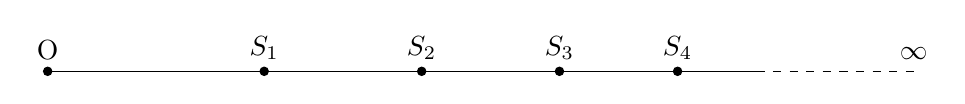
\begin{tikzpicture}
 \draw[] (0,0) -- (9,0);
  \draw[ dashed] (9,0) -- (11,0);
  
\node (o) at (0,0) [above=.2mm] {O} ; 
\node (c1) at (2.75,0)[above=.2mm]{$S_1$};
\node (c2) at (4.75,0) [above=.2mm]{$S_2$};
\node (c3) at (6.5,0) [above=.2mm]{$S_3$};
\node (c4) at (8,0) [above=.2mm] {$S_4$};
\node (inf) at (11,0) [above=.2mm]{$\infty$}; 
  \foreach \x in {0,2.75,4.75,6.5,8} 
  \draw[fill=black] (\x,0) circle (1.5pt);
\end{tikzpicture}
\vspace{1cm}
\begin{block}{Processo di Poisson non omogeneo}
\begin{itemize}
\item $(N_t)_{t\in[0,\infty)}$ Poisson non omogeneo con rate $\lambda(t)=t$
$$P\left\{N_t=n\right\}= \frac{\Lambda(t)^n}{n!} e^{-\Lambda(t)}, \quad \Lambda(t)=\int_0^t \lambda(s) ds$$
\item $\left(S_i\right)$ tempi di arrivo con densit\'a
$$f_{S_{i+1}}(t)= t \, \exp\left(-\frac{1}{2} \left(t^2 - S_i^2\right)\right), \quad \text{per } t\in [S_i,\infty )$$

\end{itemize}
\end{block}
\end{frame}


\begin{frame}{Costruzione del Brownian CRT}
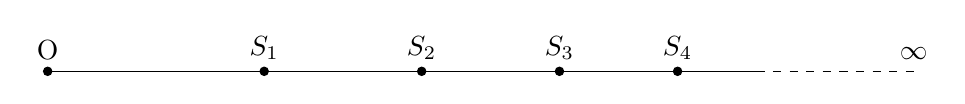
\begin{tikzpicture}
 \draw[] (0,0) -- (9,0);
  \draw[ dashed] (9,0) -- (11,0);
  
\node (o) at (0,0) [above=.2mm] {O} ; 
\node (c1) at (2.75,0)[above=.2mm]{$S_1$};
\node (c2) at (4.75,0) [above=.2mm]{$S_2$};
\node (c3) at (6.5,0) [above=.2mm]{$S_3$};
\node (c4) at (8,0) [above=.2mm] {$S_4$};
\node (inf) at (11,0) [above=.2mm]{$\infty$}; 
  \foreach \x in {0,2.75,4.75,6.5,8} 
  \draw[fill=black] (\x,0) circle (1.5pt);
\end{tikzpicture}
\begin{columns}
\begin{column}{.6 \textwidth}
\vspace{1cm}
\begin{tikzpicture}
%NODI 
\node (o) at (0,0) {O};
\node (e1) at (8,0) {$e_1$};
\node (e3) at (0,5) {$e_3$};
\node (e2) at (4,4) {$e_2$};
% ASSI
\draw[->, black] (o) -- (e1);
\draw[->, black] (o) -- (e2);
\draw[->, black] (o) -- (e3);
% PUNTINI NERI
% LABEL BRANCHPOINTS

\end{tikzpicture}
\vspace{0.01mm}
\end{column}
\begin{column}{.4 \textwidth}
%\begin{block}{Incollamento}
%$b_i$ \'e scelto uniformemente su 
%$$\bigcup\limits_{j<i} \ [[O,S_j]]$$
%\end{block}
\end{column}
\end{columns}
\end{frame}


\begin{frame}{Costruzione del Brownian CRT}
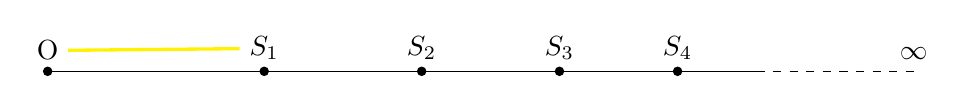
\begin{tikzpicture}
 \draw[] (0,0) -- (9,0);
  \draw[ dashed] (9,0) -- (11,0);
  
\node (o) at (0,0) [above=.2mm] {O} ; 
\node (c1) at (2.75,0)[above=.2mm]{$S_1$};
\node (c2) at (4.75,0) [above=.2mm]{$S_2$};
\node (c3) at (6.5,0) [above=.2mm]{$S_3$};
\node (c4) at (8,0) [above=.2mm] {$S_4$};
\node (inf) at (11,0) [above=.2mm]{$\infty$}; 
  \foreach \x in {0,2.75,4.75,6.5,8} 
  \draw[fill=black] (\x,0) circle (1.5pt);
 \draw [very thick, yellow] (o)--(c1);
\end{tikzpicture}

\begin{columns}
\begin{column}{.6 \textwidth}
\vspace{1cm}
\begin{tikzpicture}
%NODI 
\node (o) at (0,0) {O};
\node (s1) at (6,0) {$S_1$};
\node (e1) at (8,0) {$e_1$};
\node (e3) at (0,5) {$e_3$};
\node (e2) at (4,4) {$e_2$};
%ASSI
\draw[->, black] (s1) -- (e1);
\draw[->, black] (o) -- (e2);
\draw[->, black] (o) -- (e3);
% LINEE COLORATE
\draw[-, yellow, very thick] (o) -- (s1);
% PUNTINI NERI
% LABEL BRANCHPOINTS
\end{tikzpicture}
\vspace{0.01mm}
\end{column}
\begin{column}{.4 \textwidth}
%\begin{block}{Incollamento}
%$b_i$ \'e scelto uniformemente su 
%$$\bigcup\limits_{j<i} \ [[O,S_j]]$$
%\end{block}
\end{column}
\end{columns}
\end{frame}


\begin{frame}{Costruzione del Brownian CRT}
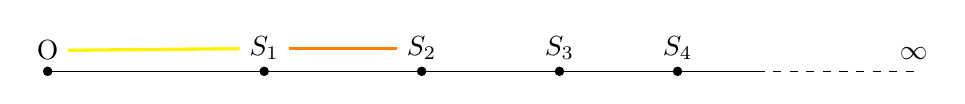
\begin{tikzpicture}
 \draw[] (0,0) -- (9,0);
  \draw[ dashed] (9,0) -- (11,0);
  
\node (o) at (0,0) [above=.2mm] {O} ; 
\node (c1) at (2.75,0)[above=.2mm]{$S_1$};
\node (c2) at (4.75,0) [above=.2mm]{$S_2$};
\node (c3) at (6.5,0) [above=.2mm]{$S_3$};
\node (c4) at (8,0) [above=.2mm] {$S_4$};
\node (inf) at (11,0) [above=.2mm]{$\infty$}; 
  \foreach \x in {0,2.75,4.75,6.5,8} 
  \draw[fill=black] (\x,0) circle (1.5pt);
 \draw [very thick, yellow] (o)--(c1);
 \draw [very thick, orange] (c1)--(c2);
\end{tikzpicture}
\begin{columns}
\begin{column}{.6 \textwidth}
\vspace{1cm}
\begin{tikzpicture}
%NODI 
\node (o) at (0,0) {O};
\node (s1) at (6,0) {$S_1$};
\node (s2) at (6,2) {$S_2$};
\node (e1) at (8,0) {$e_1$};
\node (e3) at (0,5) {$e_3$};
\node (e2) at (4,4) {$e_2$};
%ASSI
\draw[->, black] (s1) -- (e1);
\draw[->, black] (o) -- (e2);
\draw[->, black] (o) -- (e3);
% LINEE COLORATE
\draw[-, yellow, very thick] (o) -- (s1);
\draw[-, orange, very thick] (4,0) -- (s2);
% PUNTINI NERI
\draw[fill=black] (4,0) circle (1.5pt);
% LABEL BRANCHPOINTS
\node (b2) at (4,0) [below=.2mm]{$b_2$};
\end{tikzpicture}
\end{column}
\begin{column}{.4 \textwidth}
\begin{block}{Incollamento}
$b_i$ \'e scelto uniformemente su 
$$\bigcup\limits_{j<i} \ [[O,S_j]]$$
\end{block}
\end{column}
\end{columns}
\end{frame}


\begin{frame}{Costruzione del Brownian CRT}
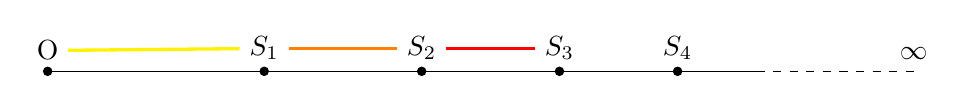
\begin{tikzpicture}
 \draw[] (0,0) -- (9,0);
  \draw[ dashed] (9,0) -- (11,0);
  
\node (o) at (0,0) [above=.2mm] {O} ; 
\node (c1) at (2.75,0)[above=.2mm]{$S_1$};
\node (c2) at (4.75,0) [above=.2mm]{$S_2$};
\node (c3) at (6.5,0) [above=.2mm]{$S_3$};
\node (c4) at (8,0) [above=.2mm] {$S_4$};
\node (inf) at (11,0) [above=.2mm]{$\infty$}; 
  \foreach \x in {0,2.75,4.75,6.5,8} 
  \draw[fill=black] (\x,0) circle (1.5pt);
 \draw [very thick, yellow] (o)--(c1);
 \draw [very thick, orange] (c1)--(c2);
  \draw [very thick, red] (c2)--(c3);  
\end{tikzpicture}
\begin{columns}
\begin{column}{.6 \textwidth}
\vspace{1cm}
\begin{tikzpicture}
%NODI 
\node (o) at (0,0) {O};
\node (s1) at (6,0) {$S_1$};
\node (s2) at (6,2) {$S_2$};
\node (s3) at (2,4) {$S_3$};
\node (e1) at (8,0) {$e_1$};
\node (e3) at (0,5) {$e_3$};
\node (e2) at (4,4) {$e_2$};
%ASSI
\draw[->, black] (s1) -- (e1);
\draw[->, black] (o) -- (e2);
\draw[->, black] (o) -- (e3);
% LINEE COLORATE
\draw[-, yellow, very thick] (o) -- (s1);
\draw[-, orange, very thick] (4,0) -- (s2);
\draw[-, red, very thick] (2,0) -- (s3);
% PUNTINI NERI
\draw[fill=black] (2,0) circle (1.5pt);
\draw[fill=black] (4,0) circle (1.5pt);
% LABEL BRANCHPOINTS
\node (b3) at (2,0) [below=.2mm]{$b_3$};
\node (b2) at (4,0) [below=.2mm]{$b_2$};
\end{tikzpicture}
\end{column}
\begin{column}{.4 \textwidth}
\begin{block}{Incollamento}
$b_i$ \'e scelto uniformemente su 
$$\bigcup\limits_{j<i} \ [[O,S_j]]$$
\end{block}
\end{column}
\end{columns}
\end{frame}


\begin{frame}{Costruzione del Brownian CRT}
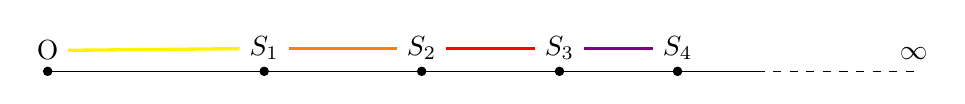
\begin{tikzpicture}
 \draw[] (0,0) -- (9,0);
  \draw[ dashed] (9,0) -- (11,0);
  
\node (o) at (0,0) [above=.2mm] {O} ; 
\node (c1) at (2.75,0)[above=.2mm]{$S_1$};
\node (c2) at (4.75,0) [above=.2mm]{$S_2$};
\node (c3) at (6.5,0) [above=.2mm]{$S_3$};
\node (c4) at (8,0) [above=.2mm] {$S_4$};
\node (inf) at (11,0) [above=.2mm]{$\infty$}; 
  \foreach \x in {0,2.75,4.75,6.5,8} 
  \draw[fill=black] (\x,0) circle (1.5pt);
 \draw [very thick, yellow] (o)--(c1);
 \draw [very thick, orange] (c1)--(c2);
  \draw [very thick, red] (c2)--(c3);
   \draw [very thick, violet] (c3)--(c4);  
\end{tikzpicture}
\begin{columns}
\begin{column}{.6 \textwidth}
\vspace{1cm}
\begin{tikzpicture}
%NODI 
\node (o) at (0,0) {O};
\node (s1) at (6,0) {$S_1$};
\node (s2) at (6,2) {$S_2$};
\node (s3) at (2,4) {$S_3$};
\node (s4) at (3,1) {$S_4$};
\node (e1) at (8,0) {$e_1$};
\node (e3) at (0,5) {$e_3$};
\node (e2) at (4,4) {$e_2$};
%ASSI
\draw[->, black] (s1) -- (e1);
\draw[->, black] (o) -- (e2);
\draw[->, black] (o) -- (e3);
% LINEE COLORATE
\draw[-, yellow, very thick] (o) -- (s1);
\draw[-, orange, very thick] (4,0) -- (s2);
\draw[-, red, very thick] (2,0) -- (s3);
\draw[dashed, violet, very thick] (5,1) -- (s4);
% PUNTINI NERI
\draw[fill=black] (2,0) circle (1.5pt);
\draw[fill=black] (4,0) circle (1.5pt);
\draw[fill=black] (5,1) circle (1.5pt);
% LABEL BRANCHPOINTS
\node (b3) at (2,0) [below=.2mm]{$b_3$};
\node (b2) at (4,0) [below=.2mm]{$b_2$};
\node (b4) at (5,1) [below right=.2mm]{$b_4$};
\end{tikzpicture}
\end{column}
\begin{column}{.4 \textwidth}
\begin{block}{Incollamento}
$b_i$ \'e scelto uniformemente su 
$$\bigcup\limits_{j<i} \ [[O,S_j]]$$
\end{block}
\end{column}
\end{columns}
\end{frame}

\begin{frame}{Costruzione del Brownian CRT}
\begin{itemize}
\item $\bullet \ T^*_{2k}$ insieme dei $k$-alberi propri
\bigskip
\item $\bullet \ \mathscr{R}_B(k):\Omega\longrightarrow T^*_{2k}\times \mathbb{R}_+^{2k-1}$ albero aleatorio ottenuto al passo $k$
\bigskip
\pause
\item $\bullet \  \mathscr{R}_B(k)$ ha densit\'a $ f\left(t,x_1, \dots x_{2k-1}\right)= s \ \exp\left(-\frac{s^2}{2}\right), \quad s=\stackrel{2k-1}{\sum\limits_{i=1}} x_i$
\bigskip
\pause
\item $\bullet \ (x_i)$ scambiabili $\implies$ $\left(\mathscr{R}_B(k)\right)_{k\in\mathbb{N}}$ consistente
\bigskip
\pause
\item $\bullet \ |S_{i+1}-S_i|\xrightarrow{P} 0 \implies \left(\mathscr{R}_B(k)\right)_{k\in\mathbb{N}}$ leaf-tight
 
\end{itemize}
\end{frame}

\begin{frame}{Costruzione del Brownian CRT}
\center Ricordando il teorema di Rappresentazione per Campionamento
\vspace{.5cm}
\begin{block}{Definizione: Brownian CRT}
\vspace{.15cm}
 $$\left(\mathscr{S}, \mu\right)\text{ \'e un Brownian CRT se}$$
 $$\forall \left(Z_i\right)_{i\in\mathbb{N}}\subseteq l_1 \text{ v.a. scambiabili con legge } \mu$$
 
 $$ r\left(\mathscr{S}, \left\{Z_1, \dots ,Z_k\right\}\right)\text{ rappresentazione insiemistica di } \mathscr{R}_B(k) \quad \forall k\in\mathbb{N}$$
 \vspace{.3cm}
\end{block}
\end{frame}


\begin{frame}{Bibliografia}
\begin{itemize}
\item $\bullet$ Aldous, D. J. \textit{The continuum random tree. I.} 1991, Ann. Probab. 19, 1-28.

\item $\bullet$ Aldous, D. J. \textit{The continuum random tree II: an overview.} 1991, Proc. Durham Symp. Stochastic Analysis 1990, 23-70. Cambridge Univ. Press.

\item $\bullet$ Aldous, D. J.  \textit{The Continuum Random Tree III.} 1993, Ann. Probab. 21, 248--289.

\item $\bullet$ Aldous, D. J. \textit{Exchangeability and related topics.} 1985, Lecture Notes in Mathematics, vol 1117. Springer, Berlin, Heidelberg.

\item $\bullet$ Patrick Billingsley, \textit{Convergence of Probability Measures.} 1968, Wiley Series in Probability and Statistics.

\end{itemize}
\end{frame}


\end{document}